%%% Presentaciones para Lenguajes de programacion y sus paradigmas 

\documentclass[xcolor=dvipsnames,table,handout]{beamer}
%\documentclass[xcolor=dvipsnames,table]{beamer}

\newcommand{\espc}{\vspace{0.3cm}}

\usepackage[utf8]{inputenc}
\usepackage[spanish]{babel}
\usepackage{hyperref}
\usepackage{lmodern}
\usepackage[T1]{fontenc}

%%%% paquetes matematicas
\usepackage{amssymb,amsmath,amscd}
\usepackage{extarrows}
\usepackage{stmaryrd}
\usepackage{mathabx}
\usepackage{mathrsfs}
% \usepackage{mathabx}
\usepackage{amsthm}

%%%%%
\usepackage{hyperref}
\usepackage{graphicx}
\usepackage{multicol}
\usepackage{pifont}
\usepackage{xcolor}
\usepackage{etex}
\usepackage{tikz}
\usepackage{array}
%\usepackage{pgfplots}

%%%% cosmetics
% D.Remy package for pretty display of rules
\usepackage{mathpartir}

% para insertar codigo con formato particular 
\usepackage{listing} 

% comillas 
\usepackage[autostyle=true,spanish=mexican]{csquotes}

% codigo 
\usepackage{verbatim}
\usepackage{alltt}

% footnotes
\usepackage[bottom]{footmisc}
\usepackage{setspace}

\usepackage{wrapfig}
\usepackage{caption}


\hfuzz=5.002pt %parameter to allow hbox overfulled by length before error!

% Options for presentation
% ------------------------
% \definecolor{mycolor}{RGB}{255,192,3}
\definecolor{mycolor}{RGB}{17,132,221}
\mode<presentation>
{
% \usetheme[secheader]{Boadilla}
% \usecolortheme{orchid}
\useoutertheme{infolines}
\useinnertheme{rectangles}
\setbeamertemplate{itemize items}[square]
\setbeamertemplate{enumerate items}[square]
\setbeamersize{text margin left=6mm, text margin right=6mm}

\setbeamercolor{alerted text}{fg=red,bg=red!70!white}
\setbeamercolor{background canvas}{bg=white}
\setbeamercolor{frametitle}{bg=mycolor,fg=white}
\setbeamercolor{normal text}{bg=white,fg=black}
\setbeamercolor{structure}{bg=black,fg=mycolor}
\setbeamercolor{title}{bg=mycolor,fg=white}
\setbeamercolor{subtitle}{bg=mycolor,fg=white}
\setbeamercolor{titlelike}{bg=white,fg=mycolor}

\setbeamercovered{invisible}

\setbeamercolor*{palette primary}{fg=mycolor,bg=white}
\setbeamercolor*{palette secondary}{bg=white,fg=white}
\setbeamercolor*{palette tertiary}{fg=mycolor,bg=white}
\setbeamercolor*{palette quaternary}{fg=white,bg=white}

\setbeamercolor{separation line}{bg=mycolor,fg=mycolor}
\setbeamercolor{fine separation line}{bg=white,fg=red}
\setbeamercolor{author in head/foot}{bg=mycolor!30!white,fg=mycolor!80!black}
\setbeamercolor{title in head/foot}{bg=mycolor!30!white,fg=mycolor!80!black}
\setbeamercolor{date in head/foot}{bg=mycolor!30!white,fg=mycolor!80!black}
\setbeamercolor{institute in head/foot}{bg=mycolor!30!white,fg=mycolor!80!black}
\setbeamercolor{section in head/foot}{bg=mycolor!60!white, fg=Red}
\setbeamercolor{subsection in head/foot}
{bg=mycolor!50!white,fg=mycolor!50!white}


\setbeamertemplate{headline}
{
  \leavevmode%
  \hbox{%
  \begin{beamercolorbox}[wd=.5\paperwidth,ht=2.65ex,dp=1.5ex,center]{section in 
head/foot}%
    \usebeamerfont{section in head/foot}\insertsectionhead\hspace*{2ex}
  \end{beamercolorbox}%
  \begin{beamercolorbox}[wd=.5\paperwidth,ht=2.65ex,dp=1.5ex,center]{subsection 
in head/foot}%
    \usebeamerfont{subsection in head/foot}\hspace*{2ex}\insertsubsectionhead
  \end{beamercolorbox}}%
  \vskip0pt%
}
% \beamerdefaultoverlayspecification{<+->}
\beamertemplatenavigationsymbolsempty
% \setbeamertemplate{footline}[frame number]
}

%%%% Macros para las notas de lenguajes de programacion


%%%% math

\newcommand{\vphi}{\varphi}
\newcommand{\vp}{\varphi}

% \newcommand{\dn}{\mathsf{DN}}
% \newcommand{\dnC}{\mathsf{DN_C}}
% \newcommand{\dnM}{\mathsf{DN_M}}
% \newcommand{\dnp}{\mathsf{DN_p}}
% \newcommand{\dnm}{\mathsf{DN_p^M}}
% \newcommand{\dnc}{\mathsf{DN_p^C}}

%\newcommand{\case}{\mathsf{case}}
%\renewcommand\labelitemi{$\circ$}

\newcommand{\imp}{\rightarrow}
\newcommand{\Imp}{\Rightarrow}
\renewcommand{\iff}{\leftrightarrow}
\newcommand{\Iff}{\Leftrightarrow}
\newcommand{\G}{\Gamma}
\newcommand{\D}{\Delta}


\newcommand{\De}{\mathcal{D}}
\newcommand{\F}{\mathcal{F}}
\newcommand{\Ge}{\mathcal{G}}
\newcommand{\Pe}{\mathcal{P}}
\newcommand{\I}{\mathcal{I}}
\newcommand{\C}{\mathcal{C}}
\newcommand{\K}{\mathcal{K}}
\renewcommand{\L}{\mathcal{L}}
\newcommand{\M}{\mathcal{M}}
\newcommand{\Nc}{\mathcal{N}}
%\newcommand{\E}{\mathcal{E}}
%\newcommand{\R}{\mathcal{R}}
%\newcommand{\Q}{\mathcal{Q}}
\newcommand{\Sc}{\mathcal{S}}
\newcommand{\Te}{\mathcal{T}}
\newcommand{\W}{\mathcal{W}}

\newcommand{\Db}{\mathbb{D}}
\newcommand{\Fb}{\mathbb{F}}
\newcommand{\Kb}{\mathbb{K}}
\newcommand{\Eb}{\mathbb{E}}
\newcommand{\Ebs}{\mathbb{E}^\star}
\newcommand{\Ob}{\mathbb{O}}
\newcommand{\Ib}{\mathbb{I}}
\newcommand{\Rb}{\mathbb{R}}
\newcommand{\Qb}{\mathbb{Q}}
\newcommand{\Kbb}{\mathbb{K}}
\newcommand{\T}{\mathbb{\Theta}}


\newcommand{\kb}{\bbkappa}

\newcommand{\Sf}{\mathsf{\Sigma}}

\newcommand{\fa}{\forall}
\newcommand{\ex}{\exists}

\newcommand{\inc}{\subseteq}

\newcommand{\Lb}{\Lambda}
\newcommand{\Om}{\Omega}
\newcommand{\lb}{\lambda}
\newcommand{\al}{\alpha}
\newcommand{\ga}{\gamma}


\newcommand{\mg}{\mathbb{m}}

\newcommand{\cg}{\mathbb{C}}
\newcommand{\dg}{\mathbb{D}}
\newcommand{\jg}{\mathbb{J}}
\newcommand{\Ha}{\mathcal{H}}
%\newcommand{\A}{\mathcal{A}}
\newcommand{\sg}{\mathbb{S}}

\newcommand{\Bc}{\mathcal{B}}
\newcommand{\Df}{\mathfrak{D}}
\newcommand{\Dc}{\mathcal{D}}
%\newcommand{\Tc}{\mathcal{T}}
\newcommand{\Mf}{\mathfrak{M}}

\newcommand{\Sg}{\mathbb{S}}

\newcommand{\Q}{\ensuremath{\mathbb{Q}}}
\newcommand{\Z}{\ensuremath{\mathbb{Z}}}
\newcommand{\N}{\ensuremath{\mathbb{N}}}
\newcommand{\R}{\ensuremath{\mathbb{R}}}
\renewcommand{\S}{\mathbb{\Sigma}}
\newcommand{\A}{\mathcal{A}}
\newcommand{\E}{\ensuremath{\exists}}
\newcommand{\iso}{\ensuremath{\cong}}
\newcommand{\union}{\ensuremath{\cup}}
\newcommand{\morinyec}{\ensuremath{\precapprox}}

\newcommand{\nin}{\ensuremath{\notin}}
\newcommand{\tog}{\makebox[7mm][l]}
\newcommand{\toge}{\makebox[11mm][l]}
\newcommand{\toget}{\makebox[13mm][l]}
\newcommand{\togeth}{\makebox[14mm][l]}
\newcommand{\togethe}{\makebox[15mm][l]}
\newcommand{\together}{\makebox[17mm][l]}
\newcommand{\niso}{\ensuremath{\not \cong}}


\newcommand{\Mg}{\mathbb{M}}
\newcommand{\Bg}{\mathbb{B}}
\newcommand{\Lg}{\mathbb{L}}
\newcommand{\Tg}{\mathbb{T}}

\newcommand{\sketch}{\Red{{\sc sketch}}}

\newcommand{\restr}[2]{#1\!\!\boldsymbol{\restriction}\!#2}

\newcommand{\vacio}{\varnothing}
\newcommand{\done}{\ensuremath{\checkmark}}

\newcommand{\ida}{$\Rightarrow \; )$ }
\newcommand{\regr}{$\Leftarrow \; )$ }

\newcommand{\ol}[1]{\overline{#1}}

\newcommand{\Tsf}{\mathsf{T}}

\newcommand{\inds}[1]{\index[simb]{#1}}

\newcommand{\B}{\mathbb{B}}
%\newcommand{\N}{\mathbb{N}}

\newcommand{\vx}{\vec{x}}
\newcommand{\vy}{\vec{y}}
\newcommand{\vz}{\vec{z}}
\newcommand{\vt}{\vec{t}}
\newcommand{\vf}{\vec{f}}


% \newcommand{\propo}{\ensuremath{\mathsf{PROP}}}
% \newcommand{\atom}{\ensuremath{\mathsf{ATOM}}}
\newcommand{\term}{\ensuremath{\mathsf{TERM}}}
\newcommand{\form}{\mathsf{FORM}}

\newcommand{\true}{\mathop{\mathsf{true}}}

%\newcommand{\id}{\mathsf{Id}}

%\newcommand{\uc}{\mathcal{U}}
%\newcommand{\Ic}{\mathcal{I}}
%\newcommand{\pc}{\mathcal{P}}
%\newcommand{\qc}{\mathcal{Q}}
%\newcommand{\mc}{\mathcal{M}}
\newcommand{\supc}{\supseteq}
\newcommand{\limo}{\mathop{\mathpzc{Lim}}}
\newcommand{\ord}{\mathsf{OR}}

\newcommand{\pt}[1]{\langle #1 \rangle}


%%%% frames
\newcommand{\titulos}[2]{\frametitle{#1}\framesubtitle{#2}}
\newcommand{\fot}[1]{\footnote{\scriptsize{#1}}}


%%%% ambientes

\newcommand{\cb}[2]{\colorbox{#1}{#2}}

\newcommand{\bc}{\begin{center}}
\newcommand{\ec}{\end{center}}
\newcommand{\be}{\begin{enumerate}}
\newcommand{\ee}{\end{enumerate}}
\newcommand{\bi}{\begin{itemize}}
\newcommand{\ei}{\end{itemize}}
\newcommand{\beq}{\begin{equation}}
\newcommand{\eeq}{\end{equation}}
\newcommand{\beqs}{\begin{equation*}}
\newcommand{\eeqs}{\end{equation*}}
\newcommand{\ba}{\begin{array}}
\newcommand{\ea}{\end{array}}


% \newtheorem{theorem}{Teorema}
% \newcommand{\teo}[1]{\begin{theorem} #1 \end{theorem}}
% \newtheorem{proposition}{Proposici\'on}
% \newcommand{\prop}[1]{\begin{proposition} #1 \end{proposition}}
% \newtheorem{definition}{Definici\'on}
% \newcommand{\defin}[1]{\begin{definition} #1 \end{definition}}
% \newtheorem{corollary}{Corolario}
% \newcommand{\cor}[1]{\begin{corollary} #1 \end{corollary}}
% \newtheorem{lemma}{Lema}
% \newcommand{\lema}[1]{\begin{lemma} #1 \end{lemma}}
% \newcommand{\dem}[1]{\begin{proof} #1 \end{proof}}

%\renewcommand{\qed}{\qedsymbol{$\mathbf{\dashv}$}}

%\newcommand{\proof}{\hfill\\\noindent\textbf{\textit{Demostraci\'on. }}}

\newcommand{\hint}{\emph{Sugerencia: }}


\newcounter{EjempCtr}[section]
\newenvironment{enumrom}{\renewcommand{\theenumi}{\roman{enumi}}%
\renewcommand{\theenumii}{\roman{enumii}}
\renewcommand{\theenumiii}{\roman{enumiii}}
\renewcommand{\theenumiv}{\roman{enumiv}}
\begin{enumerate}}{\end{enumerate}}
\newenvironment{Ejemplo}
        {\stepcounter{EjempCtr}%
        \begin{description}\item[Ejemplo \thesection.\arabic{EjempCtr}]}%
        {\end{description}}
\newenvironment{demostr}{%
             {\em Demostración:}
                \begin{quotation}}{\end{quotation}}

   \newcommand{\beje}{\begin{Ejemplo}}
\newcommand{\eeje}{\end{Ejemplo}}


\newtheorem{eje}{Ejemplo}[section]
\newcommand{\ejem}[1]{\begin{eje}\normalfont #1 \end{eje}}

% \renewcommand\contentsname{\'Indice}
%\renewcommand\chaptername{Cap\'itulo}
% \renewcommand\indexname{\'Indice}

%%\newcommand{\qed}{\hfill$\mathbb{Qed}$}
%\newcommand{\qed}{\hfill$\mathsf{\boldsymbol{\dashv}}$}
%\renewcommand{\qed}{\hfill$\boldsymbol{\dashv}$}


\newenvironment{prueba}{\vspace{-5mm}\noindent\textbf{Demostraci\'on}\\}{
\noindent$\blacksquare$\\}

\newcommand{\Ejercicios}{\section*{Ejercicios}}

 \newenvironment{manitas}{%
      \renewcommand{\labelitemi}{\ding{44}}%
      \vspace{-0.5cm}%
      \begin{itemize}%
      \setlength{\itemsep}{0pt}\setlength{\parsep}{0pt}\setlength{\topsep}{0pt}%
      }{\end{itemize}}
\newenvironment{malitos}{%
      \renewcommand{\labelitemi}%
            {\raisebox{1.5ex}{\makebox[0.3cm][l]{\begin{rotate}{-90}%
            \ding{43}\end{rotate}}}}%
      \vspace{-0.5cm}%
      \begin{itemize}%
      \setlength{\itemsep}{0pt}\setlength{\parsep}{0pt}\setlength{\topsep}{0pt}%
      }{\end{itemize}}
\newenvironment{ejercs}{
     \renewcommand{\labelenumi}{\thesection.\theenumi.-}
     \renewcommand{\labelenumii}{\theenumii)}
     \begin{enumerate}}
     {\end{enumerate}}

   \newcommand{\bej}{\begin{ejercs}}
\newcommand{\eej}{\end{ejercs}}


%\newenvironment{leterize}{%
%        \renewcommand{\theenumi}{\alph{enumi}}
%        \begin{enumerate}}{\end{enumerate}}

%\newenvironment{manitas}{%
%      \renewcommand{\labelitemi}{\ding{44}}%
%      \vspace{-0.5cm}%
%      \begin{itemize}%
%      
% \setlength{\itemsep}{0pt}\setlength{\parsep}{0pt}\setlength{\topsep}{0pt}%
%      }{\end{itemize}}



%%=============================================================================

\def\stackunder#1#2{\mathrel{\mathop{#2}\limits_{#1}}}


%%%% notas

\newcommand{\doubt}{\Red{{\LARGE {\sf ??}}}}

\newcommand{\coment}[1]{\hfill\\ \Big[{\bf Comentario Privado:} #1\Big]}
\newcommand{\preg}[1]{\hfill\\ \BrickRed{{\bf Pregunta:} #1}}
\newcommand{\conjet}[1]{\hfill\\ \OliveGreen{{\bf Conjecura:} #1}}

\newcommand{\pendiente}{\BrickRed{{\sc Pendiente}}}
\newcommand{\verifpendiente}{\BrickRed{{\sc Verificación pendiente}}}


%--------------------------------------------------------------------------

\DeclareMathAlphabet{\mathpzc}{OT1}{pzc}{m}{it}


\title[]{Lógica computacional}
\subtitle{Tema: Semántica de la Lógica de Primer Orden }
\author[]{}
\institute[UNAM-FC]{Facultad de Ciencias\\ 
Universidad Nacional Aut\'onoma de M\'exico}
\author{ Pilar Selene Linares Ar\'evalo}
\date[]{ \footnotesize{marzo 2018}
\newline{\tiny{Material desarrollado bajo el proyecto UNAM-PAPIME PE102117.}}}
 

\beamerdefaultoverlayspecification{<+->}
 
\titlegraphic{
\includegraphics[width=16mm]{fc2.png}}
 

\begin{document}

\begin{frame}
\titlepage 
\end{frame}
			
\frame{\titulos{Semántica formal}{}
\begin{block}{Interpretación (estructura)}
Sea $\L=\Pe\cup\F\cup\C$ un lenguaje o signatura de primer orden. Una 
  {\bf estructura o interpretación} para~$\L$ es un par~$\M=\pt{M,\I}$ donde 
  $M\neq\varnothing$ es un conjunto no vacío llamado el universo de la 
  estructura e $\I$ es una función con dominio~$\L$ tal que:
\bi
\item Si $P^{(n)}\in\Pe$ entonces $\I(P)$ es una relación de $m$-argumentos
  sobre $M$, es decir $\I(P)\inc M^n$. Alternativamente podemos definir la interpretación de $P$ como una función booleana que decide si una tupla está o no en la relación deseada, es decir, $\I(P): M^n \to Bool$.
\item Si $f^{(n)}\in\F$ entonces $\I(f)$ es una función con dominio $M^n$ y
  contradominio $M$, es decir\\ $\I(f):M^n\imp M$.
\item Si $c\in\C$ entonces $\I(c)$ es un elemento de $M$, es decir~$\I(c)\in M$.
\ei 
\end{block}
}

\frame{\titulos{Semántica formal}{}
Dada una interpretación $\M=\pt{M,\I}$ haremos uso de la siguiente notación :
\pause
\[
\ba{rll}
|\M| &\; =_{def} \;& M  \\ 
P^\I &\; =_{def}\;& \I(P) \\
f^\I &\; =_{def} \;& \I(f) \\ 
c^\I  &\; =_{def} \;& \I(c) 
\ea 
\]

}


\frame{\titulos{Interpretación de términos}{}
\begin{block}{Estado/ asignación}
Un {\bf estado}, asignación o valuación de las variables es una función $\sigma:\mathsf{Var}\imp M$.
\end{block}

\begin{block}{Estado modificado}
Sea  
  $\sigma:\mathsf{Var}\imp M$ un estado de las variables. Dadas las
  variables $x_1,\ldots,x_n$ y los elementos del universo $m_1,\ldots,m_n\in
  M$ definimos el {\bf estado modificado} o actualizado en $x_1,\ldots,x_n$ por
  $m_1,\ldots,m_n$ denotado $\sigma[x_1,\ldots,x_n/m_1,\ldots,m_n]$ o 
  $\sigma[\vx/\vec{m}\,]$ como sigue:
\beqs
\sigma[\vx/\vec{m}\,](y) =\left\{\ba{rl}
\sigma(y) & \mbox{si}\; y\notin\{x_1,\ldots,x_n\} \\ \\
m_i      & \mbox{si}\; y = x_i\;\;\;\;1\leq i\leq n 
\ea
\right.
\eeqs
\end{block}
}

\frame{\titulos{Interpretación de términos}{}
\begin{block}{Interpretación de términos}
Sea $\sigma$ un estado de las variables. Definimos la {\bf función de interpretación} o significado de los términos con respecto a $\sigma$, $\I_\sigma:\term\imp |\M|$ como sigue:
\[
\ba{rcl}
\I_\sigma(x) &\; = \; & \sigma(x) \\ \\ 
\I_\sigma(c) &\; = \; & \I(c) \\ \\  %= c^\I \\ 
\I_\sigma\big(f(t_1,\ldots,t_n)\big)  & \; = \; &  
f^\I(\I_\sigma(t_1),\ldots,\I_\sigma(t_n))
\ea
\]
\end{block}
}

\frame{\titulos{Interpretación de términos}{}
Hay una relación entre los estados modificados y las sustituciones: \\
\espc 
  \pause
Sup\'ongase que tenemos un t\'ermino $t$ que tiene muchas presencias de la variable $x$ y que queremos evaluar $t[x:=r]$ en alg\'un estado de cierta interpretaci\'on. \\ \espc \pause
Para ello aplicamos la definici\'on y cada vez que encontramos una presencia del subt\'ermino $r$ en $t[x:=r]$ debemos calcular el valor de $r$ en el mismo estado; lo cual es poco pr\'actico.  \\ \espc \pause

Una mejor manera de evaluar
$t[x:=r]$ ser\'{\i}a evaluar $r$ en el estado dado $\sigma$, lo cual nos da cierto
valor $m$ y evaluar el t\'ermino $t[x:=r]$ en el estado modificado
$\sigma[x/m]$. El resultado ser\'a el mismo.
}	

\frame{\titulos{Interpretación de términos}{}
\begin{exampleblock}{Lema de coincidencia para términos}
Sean $t\in\term$ y $\sigma_1,\sigma_2$ dos
  estados de las variables tales que $\sigma_1(x)=\sigma_2(x)$ para toda variable $x$
  que figura en $t$. Entonces $\I_{\sigma_1}(t)=\I_{\sigma_2}(t)$.
\end{exampleblock}
\espc
\begin{exampleblock}{Lema de sustitución para términos}
Sean $r\in\term$, $\sigma$ un estado de
  las variables, $[\vx:=\vt\;]$ una sustitución y $m_1,\ldots,m_n\in
  M$ tales que $\I_\sigma(t_i)=m_i\;\;1\leq i\leq n$. Entonces
\beqs
\I_\sigma\big(r[\vx:=\vt\;]\big) = \I_{\sigma[\vx/\vec{m}\;]}(r)
\eeqs
\end{exampleblock}
}

\frame{\titulos{Interpretación de fórmulas}{}
Ya que sabemos cómo interpretar términos, es posible definir la interpretación de fórmulas. \espc
\pause
\begin{block}{Interpretación de fórmulas I}
Sea $\sigma$ un estado de las
  variables. Definimos la {\bf función de interpretación} o significado de las
  fórmulas con respecto a $\sigma$, $\I_\sigma:\form\imp\{0,1\}$ como sigue:
\[
\ba{lcl}
\I_\sigma(\bot) \; = \;  0  &  \I_\sigma(\top) \; = \;  1  & \\ \\ \pause
\I_\sigma\big(P(t_1,\ldots,t_m)\big)\; = \;1 & \;\mbox{si y sólo si}\; &
\big(\I_\sigma(t_1),\ldots,\I_\sigma(t_m)\big)\in P^\I \\ \\ \pause
\I_\sigma(t_1=t_2) \; = \;  1 & \;\mbox{si y sólo si}\; & \I_\sigma(t_1)=\I_\sigma(t_2) \\ \\
\ea
\]
\end{block}
}


\frame{\titulos{Interpretación de fórmulas}{}
\begin{block}{Interpretación de fórmulas II}
Sea $\sigma$ un estado de las
  variables. Definimos la {\bf función de interpretación} o significado de las
  fórmulas con respecto a $\sigma$, $\I_\sigma:\form\imp\{0,1\}$ como sigue:
\[
\ba{lcl}
\I_\sigma(\neg\vp) \; = \; 1 & \;\mbox{si y sólo si}\; & \I_\sigma(\vp)=0 \\ \\ \pause
\I_\sigma(\vp\land\psi) \; = \;  1 & \;\mbox{si y sólo si}\; &
\I_\sigma(\vp)=\I_\sigma(\psi)=1 \\ \\ \pause
\I_\sigma(\vp\lor\psi) \; = \;  0 & \;\mbox{si y sólo si}\; &
\I_\sigma(\vp)=\I_\sigma(\psi)=0 \\ \\ \pause
\I_\sigma(\vp\imp\psi) \; = \;  0 & \;\mbox{si y sólo si}\; &
\I_\sigma(\vp)=1\;\mbox{e}\;\I_\sigma(\psi)=0 \\ \\ \pause
\I_\sigma(\vp\iff\psi) \; = \;  1 & \;\mbox{si y sólo si}\; &
\I_\sigma(\vp)=\I_\sigma(\psi) \\ \\

\ea
\]
\end{block}
}

\frame{\titulos{Interpretación de fórmulas}{}
\begin{block}{Interpretación de fórmulas III}
Sea $\sigma$ un estado de las
  variables. Definimos la {\bf función de interpretación} o significado de las
  fórmulas con respecto a $\sigma$, $\I_\sigma:\form\imp\{0,1\}$ como sigue:
\[
\ba{lcl}
\I_\sigma(\fa x\vp) \; = \;  1 & \;\mbox{si y sólo si}\; &
\I_{\sigma[x/m]}(\vp)=1\;\;\mbox{para todo}\;m\in M \\ \\ \pause
\I_\sigma(\ex x\vp) \; = \;  1 & \;\mbox{si y sólo si}\; &
\I_{\sigma[x/m]}(\vp)=1\;\;\mbox{para algún}\;m\in M \\ \\
\ea
\]
\end{block}
}

\frame{\titulos{Interpretación de fórmulas}{}
Análogamente al caso de términos se cumplen los lemas de coincidencia y
sustitución. \espc \pause
\begin{exampleblock}{Lema de coincidencia para fórmulas}
Sean $\vp$ una fórmula y 
$\sigma_1,\sigma_2$ dos estados de las variables tales que 
$\sigma_1(x)=\sigma_2(x)$ para toda variable
$x\in FV(\vp)$. Entonces $\I_{\sigma_1}(\vp)=\I_{\sigma_2}(\vp)$.
\end{exampleblock}
\pause
\espc
\begin{exampleblock}{Lema de sustitución para fórmulas}
Sean $\vp\in\form$, $\sigma$ un estado 
  de las variables, \\$[\vx:=\vt\;]$ una sustitución y $m_1,\ldots,m_n\in M$ 
  tales que $m_i=\I_\sigma(t_i)\;\;1\leq i\leq n$. Entonces
\[
\I_\sigma\big(\vp[\vx:=\vt\;]\big) = \I_{\sigma[\vx/\vec{m}\;]}(\vp) 
\]
\end{exampleblock}

}

\frame{\titulos{Interpretación de fórmulas}{}
\begin{block}{Satisfacibilidad, verdad y falsedad.}
Sean $\vp$ una fórmula y $\M=\pt{M,\I}$ una 
interpretación. Entonces
\bi
\item $\vp$ es {\bf satisfacible} en $\M$ si existe un estado de las variables $\sigma$ tal que $\I_\sigma(\vp)=1$, lo cual suele
  denotarse con $\M\models\vp[\sigma]$ o con $\M\models_\sigma\vp$.  
\item $\vp$ es {\bf verdadera} en $\M$ si para todo estado de las variables $\sigma$  se tiene $\I_\sigma(\vp)=1$, es decir, si $\vp$ es satisfacible en $\M$ en todos los estados posibles. \\
En tal caso también decimos que $\M$ es un {\bf modelo} de $\vp$ lo cual se
  denotará con $\M\models\vp$.
\item $\vp$ es {\bf falsa} en $\M$ si y sólo si $\M\models\neg\vp$. Es decir $\vp$ es falsa 
si y sólo si su negación $\neg\vp$ es verdadera.
\ei
\end{block}
}

\frame{\titulos{Interpretación de fórmulas}{}
¡En lógica de predicados decir que $\varphi$ es falsa y no es verdadera NO es lo mismo!. \\
\pause

\bi
\item Si $\vp$ no es verdadera (es decir, si~$\M\not\models\vp$), entonces existe un estado~$\sigma$ tal que 
$\M\not\models_\sigma\vp$, es decir $\I_\sigma(\vp)=0$ o bien $\vp$ es  insatisfacible en el estado~$\sigma$.

\item Una fórmula no verdadera es  aquella tal que es insatisfacible en algún estado de sus variables, o bien tal que su negación es satisfacible en algún estado de sus variables. 

\item Para poder afirmar que  $\vp$ es falsa, tendríamos que mostrar que $\M\models\neg\vp$, es decir  que~$\neg\vp$ es satisfacible en \textbf{todos} los estados posibles. 
\ei

\pause
\setbeamercolor{postit}{bg=yellow!50!white}
\begin{beamercolorbox}{postit}
Si una fórmula~$\vp$ no es verdadera, no podemos concluir que $\vp$ es falsa.
\end{beamercolorbox}

}

\frame{\titulos{Interpretación de fórmulas}{}
\begin{figure}[t]
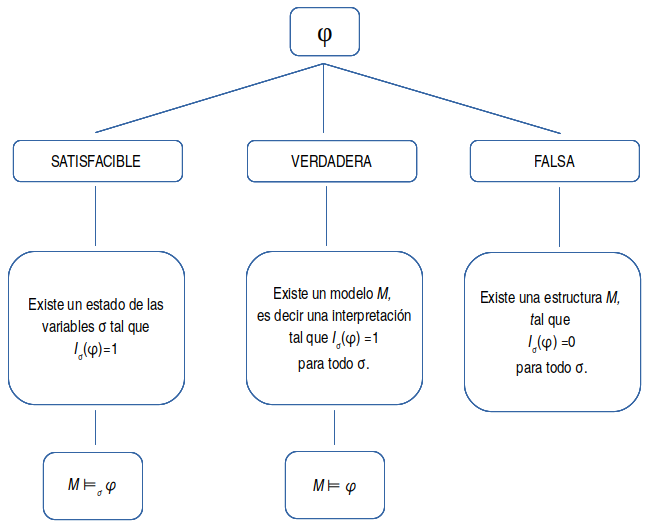
\includegraphics[width=8cm]{diagrama}
\centering
\end{figure}
}

\frame{\titulos{Propiedades noción verdad}{}
La relaci\'on de verdad en lógica de predicados no tiene las mismas propiedades que su contraparte en la lógica proposicional, propiedades que sí hereda la relación de satisfacibilidad. \\
\espc
\pause
Sean $\L=\{P^{(1)},Q^{(1)}\},\;\M=\langle \mathbb{N},\I\rangle$  donde $P^\I$ es la propiedad \enquote{ser par} y $Q^\I$ es la
propiedad \enquote{ser impar}. \\
\espc
\pause
Entonces $\M\models P(x)\lor Q(x)$ puesto que cualquier n\'umero natural es
par o es impar. \\ \pause
Sin embargo no se cumple que $\M\models P(x)$ ni que $\M\models Q(x)$. Puesto 
que el valor de~$x$ no puede ser siempre par o siempre impar.

\pause
\espc
\setbeamercolor{postit}{bg=yellow!50!white}
\begin{beamercolorbox}{postit}
Observemos que si una disyunción es verdadera en $\M$ entonces no necesariamente lo es alguna de sus subf\'ormulas.
Es decir, $\M\models \vp\lor\psi$ no implica que $\M\models\vp$ o 
$\M\models\psi$.
\end{beamercolorbox}
}

\frame{\titulos{Propiedades noción verdad}{}
Veamos ahora algunas propiedades de la relaci\'on de verdad.
\begin{exampleblock}{}
Sean $\M$ una $\L$-interpretaci\'on y $\vp,\psi$ f\'ormulas. Entonces
\bi
\item Si $\M\models\vp$ entonces $\M\not\models\neg\vp$.
\item Si $\M\models\vp\imp\psi$ y $\M\models\vp$ entonces
  $\M\models\psi$.
\item Si $\M\models\vp$ entonces $\M\models\vp\lor\psi$.
  \item $\M\models\vp\land\psi$ si y sólo si $\M\models\vp$ y $\M\models\psi$.
\item $\M\models\vp\;\mbox{si y sólo si}\;\M\models\fa\vp.$ donde
  $\fa\vp$ denota a la cerradura universal de $\vp$, es decir a la
  fórmula obtenida al cuantificar universalmente todas las variables
  libres de $\vp$.
  
\ei
\end{exampleblock}
}


%\frame{\titulos{}{}
%\begin{block}{}
%
%\end{block}
%}
%
%\frame{\titulos{}{}
%\begin{exampleblock}{}
%
%\end{exampleblock}
%}
%
%\frame{\titulos{}{}
%
%}



\end{document}
